%\emph{Analysis: any disambiguations of the  case  description and assumptions made, any potentially added requirements}

During the requirement analysis of the challenge, the foundation of our reflections and modeling intentions is guided by the general model federation approach.

In a first step, the federation approach is mainly based on modeling relationships between several models, independently of their abstraction level and the model architecture.

During the next step of our approach, we try to take into account the reusability of the relationships by identifying the semantics of them. The goal is the identification of concepts with their behavior. The last step is to organize or structure these concepts to improve reusability and extensibility, to create virtual models in \FML terminology.

Like in a lot of modeling approaches, these  steps could also be achieved in any order and iteratively. But our goal during the challenge's analysis remains to produce a \FML virtual model architecture for our federation.
As shown in the figure~\ref{fig:MultilevelArchitecture}, we defined two virtual models (Base and Acme processes abstractions) instantiated by two virtual model instances (XSure and Acme processes). As the figure shows the virtual models play the role of metamodels, in the sense of concept definition with a level-agnostic approach. The virtual model instances play the role of models conforming to the metamodel definitions. In the rest of the paper, we use the term metamodel and model to simplify the presentation.
The resulting architecture follows the way the challenge is presented and this
organization allows for the possibility of flexible extensions.


\begin{figure}[t]
    \centering
    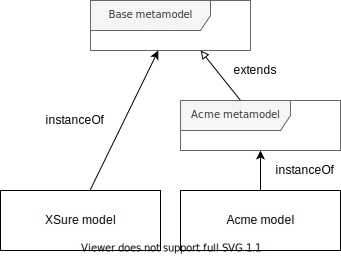
\includegraphics[width=0.7 \columnwidth]{Figures/MultilevelArchitecture.pdf}
    \caption{Multilevel architecture of our solution}
    \label{fig:MultilevelArchitecture}
\end{figure}

Our analysis of the use case leads to identify two main modeling axes (as presented in the figure \ref{fig:LinguisticAndOntologicInstantiation}):
\begin{itemize}
    \item The horizontal axis is characterized as the ontological instantiation axis, in the sense that the domain type definition (\ie \texttt{ProcessType}) is referenced by an instance definition (\ie \texttt{Process}). In our base metamodel, each domain type definition is referenced by its instance definition, as developed in the section \ref{sec:ProcessEnactment}

\item The vertical axis is viewed as the linguistic instantiation, relative to the use of the \FML language. The virtual model, defined as the core definition metamodel, generates a model founded on the instantiation mechanism of the \FML Language. This mechanism is similar to the classical object/instance mechanism of the object languages but without any constraint on the referenced virtual model, \ie metamodel. The set of resulting instances comes from several virtual models
of any abstraction level as detailed in the section. \ref{sec:AcmeSoftwareDevelopmentProcess}


\end{itemize}

\begin{figure}
    \centering
    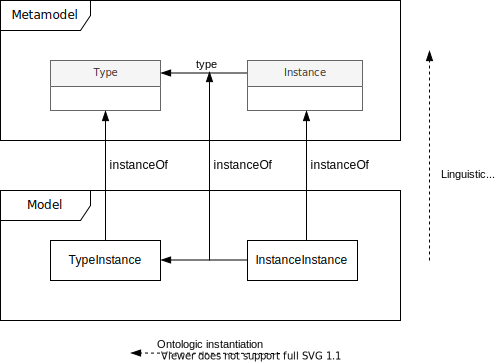
\includegraphics[width=1.0 \columnwidth]{Figures/Instantiation.pdf}
    \caption{Problem  Domain Linguistic and ontologic instantiation}
    \label{fig:LinguisticAndOntologicInstantiation}
\end{figure}

Based on this approach, we organize our set of models following the architecture of the aforementioned Figure \ref{fig:MultilevelArchitecture}. The resulting multi-level architecture is organized in two virtual models, one for the core concepts metamodel containing the definition of Processes and Tasks, and one, the Acme metamodel, extending the previous model to integrate the Acme definitions. The \FML language defines multiple inheritance concept between virtual models as illustrated in the section~\ref{sec:AcmeSoftwareDevelopmentProcess}.

Finally, as explained previously, the defined level for the Acme  and the XSure models is the result of the instantiation of virtual models. In our approach this virtual model instance level can't be specialized or extended but all the other virtual models could be extended by any concepts, as a new federated model.
Also, the instance level can be instantiated from any virtual model, which represents any metamodel level.

%\noteAntoine{Pourquoi S9 et S13 sont ambigus, quels choix on a fait...}
%\todo[inline]{noms pas dans la spec, complètement implicite ; }

%We now analyse a few specifications that deserve a comment for the choices we made.

%\begin{itemize}
%    \item We added an implicit specification (S0) saying that all things have names.
%    \item (S9) It is unclear when a tested artefact must be associated to its test report. At the creation of the artefact or of its report? \todo[inline]{We choose\dots}
%    \item (S13) [linked to P9] \todo[inline]{We choose to interpret \dots}
%\end{itemize}

%The analysis of the specification should be presented in this section. However, t
The choices we made are complicated to justify out of context. That is why our choices are presented within the next section model presentation.

% cross level constraints or added models as federated metamodels


%\todo[inline]{quelles hypothèses supplémentaires ?}
%\todo[inline]{+ architecture de la modélisation (ce qui se trouve dans le ppt), le détail se retrouvera dans la section suivante}
